% Options for packages loaded elsewhere
\PassOptionsToPackage{unicode}{hyperref}
\PassOptionsToPackage{hyphens}{url}
\PassOptionsToPackage{dvipsnames,svgnames,x11names}{xcolor}
%
\documentclass[
  letterpaper,
  DIV=11,
  numbers=noendperiod]{scrartcl}

\usepackage{amsmath,amssymb}
\usepackage{iftex}
\ifPDFTeX
  \usepackage[T1]{fontenc}
  \usepackage[utf8]{inputenc}
  \usepackage{textcomp} % provide euro and other symbols
\else % if luatex or xetex
  \usepackage{unicode-math}
  \defaultfontfeatures{Scale=MatchLowercase}
  \defaultfontfeatures[\rmfamily]{Ligatures=TeX,Scale=1}
\fi
\usepackage{lmodern}
\ifPDFTeX\else  
    % xetex/luatex font selection
\fi
% Use upquote if available, for straight quotes in verbatim environments
\IfFileExists{upquote.sty}{\usepackage{upquote}}{}
\IfFileExists{microtype.sty}{% use microtype if available
  \usepackage[]{microtype}
  \UseMicrotypeSet[protrusion]{basicmath} % disable protrusion for tt fonts
}{}
\makeatletter
\@ifundefined{KOMAClassName}{% if non-KOMA class
  \IfFileExists{parskip.sty}{%
    \usepackage{parskip}
  }{% else
    \setlength{\parindent}{0pt}
    \setlength{\parskip}{6pt plus 2pt minus 1pt}}
}{% if KOMA class
  \KOMAoptions{parskip=half}}
\makeatother
\usepackage{xcolor}
\setlength{\emergencystretch}{3em} % prevent overfull lines
\setcounter{secnumdepth}{5}
% Make \paragraph and \subparagraph free-standing
\ifx\paragraph\undefined\else
  \let\oldparagraph\paragraph
  \renewcommand{\paragraph}[1]{\oldparagraph{#1}\mbox{}}
\fi
\ifx\subparagraph\undefined\else
  \let\oldsubparagraph\subparagraph
  \renewcommand{\subparagraph}[1]{\oldsubparagraph{#1}\mbox{}}
\fi

\usepackage{color}
\usepackage{fancyvrb}
\newcommand{\VerbBar}{|}
\newcommand{\VERB}{\Verb[commandchars=\\\{\}]}
\DefineVerbatimEnvironment{Highlighting}{Verbatim}{commandchars=\\\{\}}
% Add ',fontsize=\small' for more characters per line
\usepackage{framed}
\definecolor{shadecolor}{RGB}{241,243,245}
\newenvironment{Shaded}{\begin{snugshade}}{\end{snugshade}}
\newcommand{\AlertTok}[1]{\textcolor[rgb]{0.68,0.00,0.00}{#1}}
\newcommand{\AnnotationTok}[1]{\textcolor[rgb]{0.37,0.37,0.37}{#1}}
\newcommand{\AttributeTok}[1]{\textcolor[rgb]{0.40,0.45,0.13}{#1}}
\newcommand{\BaseNTok}[1]{\textcolor[rgb]{0.68,0.00,0.00}{#1}}
\newcommand{\BuiltInTok}[1]{\textcolor[rgb]{0.00,0.23,0.31}{#1}}
\newcommand{\CharTok}[1]{\textcolor[rgb]{0.13,0.47,0.30}{#1}}
\newcommand{\CommentTok}[1]{\textcolor[rgb]{0.37,0.37,0.37}{#1}}
\newcommand{\CommentVarTok}[1]{\textcolor[rgb]{0.37,0.37,0.37}{\textit{#1}}}
\newcommand{\ConstantTok}[1]{\textcolor[rgb]{0.56,0.35,0.01}{#1}}
\newcommand{\ControlFlowTok}[1]{\textcolor[rgb]{0.00,0.23,0.31}{#1}}
\newcommand{\DataTypeTok}[1]{\textcolor[rgb]{0.68,0.00,0.00}{#1}}
\newcommand{\DecValTok}[1]{\textcolor[rgb]{0.68,0.00,0.00}{#1}}
\newcommand{\DocumentationTok}[1]{\textcolor[rgb]{0.37,0.37,0.37}{\textit{#1}}}
\newcommand{\ErrorTok}[1]{\textcolor[rgb]{0.68,0.00,0.00}{#1}}
\newcommand{\ExtensionTok}[1]{\textcolor[rgb]{0.00,0.23,0.31}{#1}}
\newcommand{\FloatTok}[1]{\textcolor[rgb]{0.68,0.00,0.00}{#1}}
\newcommand{\FunctionTok}[1]{\textcolor[rgb]{0.28,0.35,0.67}{#1}}
\newcommand{\ImportTok}[1]{\textcolor[rgb]{0.00,0.46,0.62}{#1}}
\newcommand{\InformationTok}[1]{\textcolor[rgb]{0.37,0.37,0.37}{#1}}
\newcommand{\KeywordTok}[1]{\textcolor[rgb]{0.00,0.23,0.31}{#1}}
\newcommand{\NormalTok}[1]{\textcolor[rgb]{0.00,0.23,0.31}{#1}}
\newcommand{\OperatorTok}[1]{\textcolor[rgb]{0.37,0.37,0.37}{#1}}
\newcommand{\OtherTok}[1]{\textcolor[rgb]{0.00,0.23,0.31}{#1}}
\newcommand{\PreprocessorTok}[1]{\textcolor[rgb]{0.68,0.00,0.00}{#1}}
\newcommand{\RegionMarkerTok}[1]{\textcolor[rgb]{0.00,0.23,0.31}{#1}}
\newcommand{\SpecialCharTok}[1]{\textcolor[rgb]{0.37,0.37,0.37}{#1}}
\newcommand{\SpecialStringTok}[1]{\textcolor[rgb]{0.13,0.47,0.30}{#1}}
\newcommand{\StringTok}[1]{\textcolor[rgb]{0.13,0.47,0.30}{#1}}
\newcommand{\VariableTok}[1]{\textcolor[rgb]{0.07,0.07,0.07}{#1}}
\newcommand{\VerbatimStringTok}[1]{\textcolor[rgb]{0.13,0.47,0.30}{#1}}
\newcommand{\WarningTok}[1]{\textcolor[rgb]{0.37,0.37,0.37}{\textit{#1}}}

\providecommand{\tightlist}{%
  \setlength{\itemsep}{0pt}\setlength{\parskip}{0pt}}\usepackage{longtable,booktabs,array}
\usepackage{calc} % for calculating minipage widths
% Correct order of tables after \paragraph or \subparagraph
\usepackage{etoolbox}
\makeatletter
\patchcmd\longtable{\par}{\if@noskipsec\mbox{}\fi\par}{}{}
\makeatother
% Allow footnotes in longtable head/foot
\IfFileExists{footnotehyper.sty}{\usepackage{footnotehyper}}{\usepackage{footnote}}
\makesavenoteenv{longtable}
\usepackage{graphicx}
\makeatletter
\def\maxwidth{\ifdim\Gin@nat@width>\linewidth\linewidth\else\Gin@nat@width\fi}
\def\maxheight{\ifdim\Gin@nat@height>\textheight\textheight\else\Gin@nat@height\fi}
\makeatother
% Scale images if necessary, so that they will not overflow the page
% margins by default, and it is still possible to overwrite the defaults
% using explicit options in \includegraphics[width, height, ...]{}
\setkeys{Gin}{width=\maxwidth,height=\maxheight,keepaspectratio}
% Set default figure placement to htbp
\makeatletter
\def\fps@figure{htbp}
\makeatother

\KOMAoption{captions}{tableheading}
\makeatletter
\@ifpackageloaded{caption}{}{\usepackage{caption}}
\AtBeginDocument{%
\ifdefined\contentsname
  \renewcommand*\contentsname{Table of contents}
\else
  \newcommand\contentsname{Table of contents}
\fi
\ifdefined\listfigurename
  \renewcommand*\listfigurename{List of Figures}
\else
  \newcommand\listfigurename{List of Figures}
\fi
\ifdefined\listtablename
  \renewcommand*\listtablename{List of Tables}
\else
  \newcommand\listtablename{List of Tables}
\fi
\ifdefined\figurename
  \renewcommand*\figurename{Figure}
\else
  \newcommand\figurename{Figure}
\fi
\ifdefined\tablename
  \renewcommand*\tablename{Table}
\else
  \newcommand\tablename{Table}
\fi
}
\@ifpackageloaded{float}{}{\usepackage{float}}
\floatstyle{ruled}
\@ifundefined{c@chapter}{\newfloat{codelisting}{h}{lop}}{\newfloat{codelisting}{h}{lop}[chapter]}
\floatname{codelisting}{Listing}
\newcommand*\listoflistings{\listof{codelisting}{List of Listings}}
\makeatother
\makeatletter
\makeatother
\makeatletter
\@ifpackageloaded{caption}{}{\usepackage{caption}}
\@ifpackageloaded{subcaption}{}{\usepackage{subcaption}}
\makeatother
\ifLuaTeX
  \usepackage{selnolig}  % disable illegal ligatures
\fi
\usepackage{bookmark}

\IfFileExists{xurl.sty}{\usepackage{xurl}}{} % add URL line breaks if available
\urlstyle{same} % disable monospaced font for URLs
\hypersetup{
  pdftitle={Popularity and Attendance of Aquatics Recreation Courses},
  pdfauthor={-Luka Tosic},
  colorlinks=true,
  linkcolor={blue},
  filecolor={Maroon},
  citecolor={Blue},
  urlcolor={Blue},
  pdfcreator={LaTeX via pandoc}}

\title{Popularity and Attendance of Aquatics Recreation
Courses\thanks{Code and data are available at:
https://github.com/LukaTosic09/Recreation\_Programs\_EDA}}
\author{-Luka Tosic}
\date{September 26, 2024}

\begin{document}
\maketitle
\begin{abstract}
This paper analyzes the relationship between course size and attendance
for aquatic courses offered by the City of Toronto's Parks Forestry and
Recreation (PFR) commission. The top finding shows that student
attendance is highest in \_\_\_\_\_ courses. Third sentence. Further
analysis would look at where courses have higher or lower engagement,
and would look at when attendance begins to drop across cours.
\end{abstract}

\begin{Shaded}
\begin{Highlighting}[]
\CommentTok{\#init chunk}
\CommentTok{\#| include: false}
\CommentTok{\#| warning: false}
\CommentTok{\#| message: false}
\CommentTok{\#| echo: false}

\FunctionTok{library}\NormalTok{(tidyverse)}
\end{Highlighting}
\end{Shaded}

\begin{verbatim}
-- Attaching core tidyverse packages ------------------------ tidyverse 2.0.0 --
v dplyr     1.1.4     v readr     2.1.5
v forcats   1.0.0     v stringr   1.5.1
v ggplot2   3.5.1     v tibble    3.2.1
v lubridate 1.9.3     v tidyr     1.3.1
v purrr     1.0.2     
-- Conflicts ------------------------------------------ tidyverse_conflicts() --
x dplyr::filter() masks stats::filter()
x dplyr::lag()    masks stats::lag()
i Use the conflicted package (<http://conflicted.r-lib.org/>) to force all conflicts to become errors
\end{verbatim}

\begin{Shaded}
\begin{Highlighting}[]
\FunctionTok{library}\NormalTok{(dplyr)}
\FunctionTok{library}\NormalTok{(knitr)}

\NormalTok{data }\OtherTok{\textless{}{-}} \FunctionTok{read.csv}\NormalTok{(}\StringTok{"../data/raw\_data/unedited\_data.csv"}\NormalTok{)}
\end{Highlighting}
\end{Shaded}

\section{Introduction}\label{introduction}

For the City of Toronto's Parks Forestry and Recreation (PFR)
Commission's swim instructors and for patrons, course sizes are a
constant point of debate. I am a swim instructor for PFR and I am
interested in analyzing the popularity and student retention across
different courses; as well as analyzing course availability and
popularity across the city.

\section{Data}\label{data}

The data is taken from (opendatatoronto), it is the Recreational Courses
Historical Data dataset. It was cleaned using BaseR, (dplyr) and
(tidyverse) packages and visualizations are done with (ggplot).

Relevant features of the data include categorization by ward and
district, classification as drop in or sign up (regular), number of
participants registered, the number of classes, the number of
participants registered and the number of total visits to a course.

We can't see attendance for each class, but we have the total attendance
given by Visits, and the Number\_of\_Classes to give us a mean visits
per week. We can plot the number of students registered vs mean visits
over a session. Since the number of students attending each class can't
exceed the number registered, if we make a scatter plot and fit a linear
model using ggplot, we can expect a slope of at most 1.

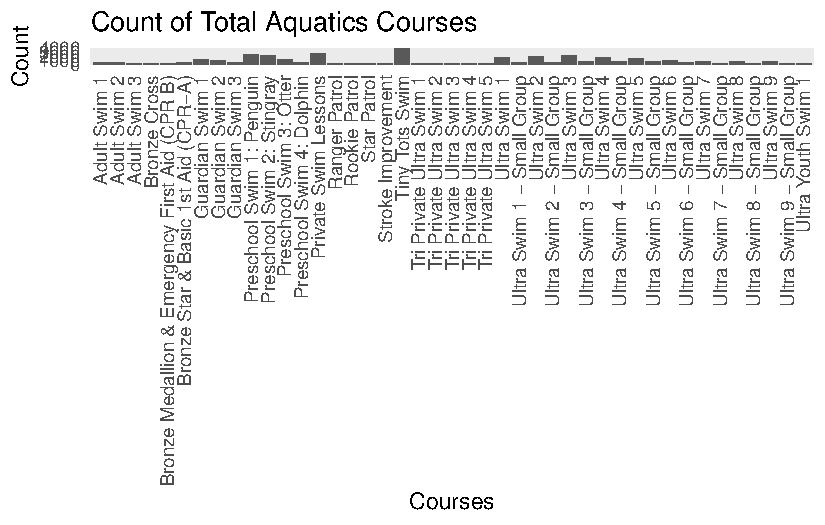
\includegraphics{paper_files/figure-pdf/unnamed-chunk-2-1.pdf}

\newpage

Tiny Tots Swim is by far the most offered in the city, this makes sense
as the classes are only 15 minutes as opposed to all other classes which
are 30 minutes or longer, so more can be offered in a single day;
moreover, Tiny Tots can be run at any pool including wading pools which
increases the number of facilities that can host it. We can also see
that the small group ultra 1-9 swims are offered anywhere from twice to
five times less often than their regular counterparts. The tri private
swims are 3-student courses offered most commonly at Douglas Snow
Aquatic Centre and Matty Eckler Recreation Centre, both in the North
District of the city.

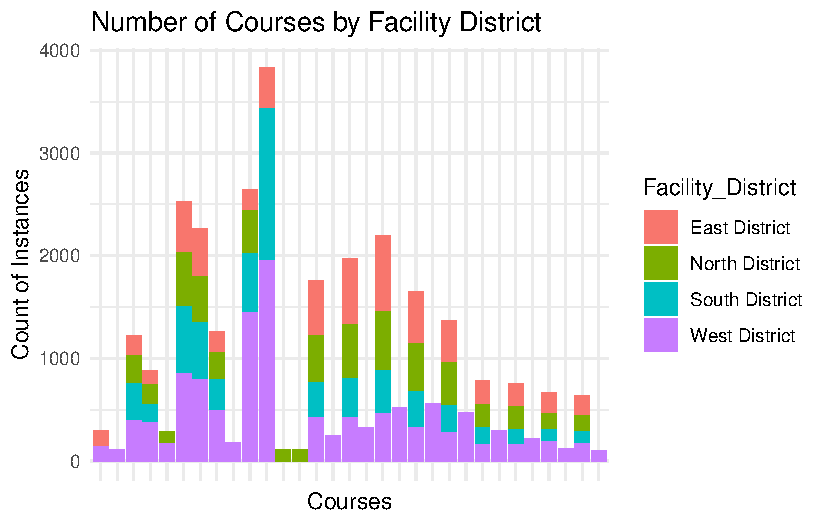
\includegraphics{paper_files/figure-pdf/unnamed-chunk-3-1.pdf}

\section{Discussion}\label{discussion}

\begin{verbatim}
`geom_smooth()` using formula = 'y ~ x'
\end{verbatim}

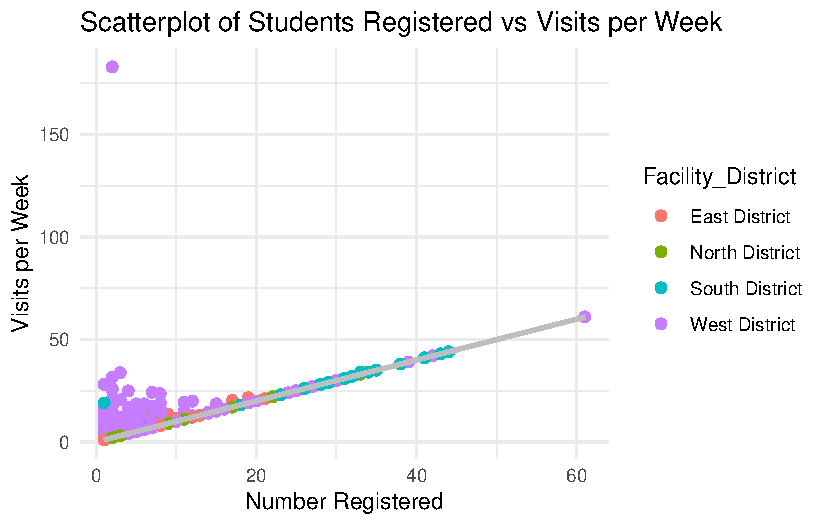
\includegraphics{paper_files/figure-pdf/unnamed-chunk-4-1.pdf}

\begin{Shaded}
\begin{Highlighting}[]
\FunctionTok{ggplot}\NormalTok{(aquatics\_data }\SpecialCharTok{|\textgreater{}} \FunctionTok{filter}\NormalTok{(Response }\SpecialCharTok{\textless{}=}\NormalTok{ Course\_Reg), }\FunctionTok{aes}\NormalTok{(}\AttributeTok{x =}\NormalTok{ Course\_Reg, }\AttributeTok{y =}\NormalTok{ Response)) }\SpecialCharTok{+}
  \FunctionTok{geom\_point}\NormalTok{(}\AttributeTok{color =} \StringTok{"black"}\NormalTok{, }\AttributeTok{size =} \DecValTok{2}\NormalTok{) }\SpecialCharTok{+}  
  \FunctionTok{geom\_smooth}\NormalTok{(}\AttributeTok{method =} \StringTok{"lm"}\NormalTok{, }\AttributeTok{color =} \StringTok{"red"}\NormalTok{, }\AttributeTok{se =} \ConstantTok{FALSE}\NormalTok{) }\SpecialCharTok{+}  
  \FunctionTok{labs}\NormalTok{(}
    \AttributeTok{title =} \StringTok{"Scatterplot of Students Registered vs Visits per Week"}\NormalTok{,}
    \AttributeTok{x =} \StringTok{"Number Registered"}\NormalTok{,}
    \AttributeTok{y =} \StringTok{"Visits per Week"}
\NormalTok{  ) }\SpecialCharTok{+}
  \FunctionTok{theme\_minimal}\NormalTok{()}
\end{Highlighting}
\end{Shaded}

\begin{verbatim}
`geom_smooth()` using formula = 'y ~ x'
\end{verbatim}

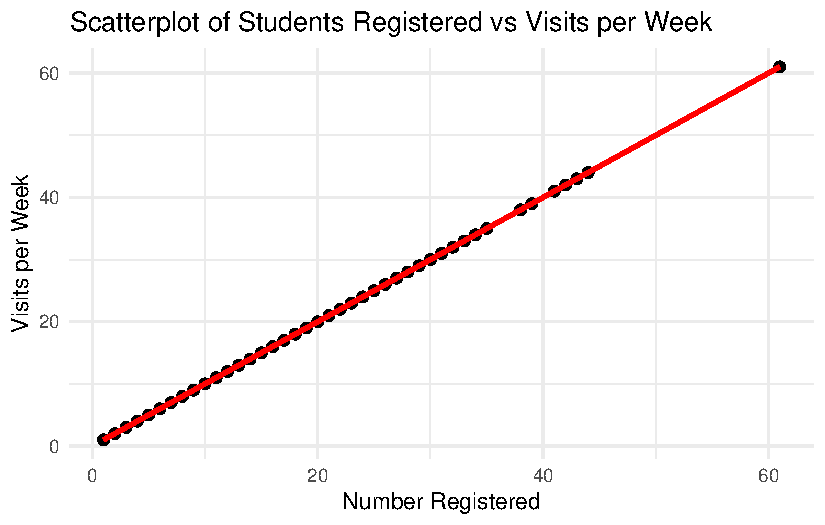
\includegraphics{paper_files/figure-pdf/unnamed-chunk-5-1.pdf}

\begin{Shaded}
\begin{Highlighting}[]
\FunctionTok{glimpse}\NormalTok{(aquatics\_data)}
\end{Highlighting}
\end{Shaded}

\begin{verbatim}
Rows: 36,316
Columns: 37
$ X                 <int> 1, 7, 40, 41, 42, 43, 60, 195, 196, 197, 198, 202, 2~
$ Course_Barcode    <int> 2644565, 2728170, 2716397, 2656342, 2699430, 2698036~
$ Program           <chr> "Ultra Swim 3", "Tiny Tots Swim", "Aquafit - Adult",~
$ Course            <chr> "Ultra Swim 3", "Tiny Tots Swim", "Aquafit: Sports C~
$ Section           <chr> "Swimming", "Swimming", "Swimming", "Swimming", "Swi~
$ SubSection        <chr> "Child/Youth", "Early Child", "Adult", "Adult", "Adu~
$ Location          <chr> "Parkdale Community Recreation Centre", "Toronto Pan~
$ Facility_District <chr> "South District", "East District", "West District", ~
$ Facility_Type     <chr> "Pool - Indoor - B", "Pool-Indoor", "Pool - Indoor -~
$ Postal_Code       <chr> "M6K 2W1", "M1C 0C7", "M8X 1Z4", "M4C 5T3", "M4C 5T3~
$ Ward              <int> 14, 44, 5, 32, 32, 32, 32, 12, 12, 12, 12, 17, 17, 2~
$ Facility          <chr> "Pool (B)", "Training Pool - Shallow Lane 6", "Pool ~
$ Min_Age           <dbl> 5, 1, 17, 17, 17, 17, 17, 17, 17, 17, 17, 3, 3, 13, ~
$ Max_Age           <dbl> 120, 5, 120, 120, 120, 120, 120, 120, 120, 120, 120,~
$ Min_Reg           <int> 3, 1, 10, 10, 5, 10, 10, 8, 8, 8, 8, 2, 2, 4, 6, 6, ~
$ Max_Reg           <int> 6, 1, 15, 40, 35, 40, 30, 25, 25, 25, 25, 4, 4, 10, ~
$ Number_of_Classes <int> 9, 9, 9, 24, 18, 24, 24, 9, 9, 9, 9, 8, 9, 9, 9, 8, ~
$ Days_of_the_Week  <chr> "Sa", "Sa", "Th", "Tu, Th", "Tu, Th", "Tu, Th", "Tu,~
$ Reg_Session       <chr> "Winter", "Winter", "Summer", "Winter", "Summer", "S~
$ Session_Year      <int> 2015, 2015, 2015, 2015, 2015, 2015, 2015, 2015, 2015~
$ Course_Reg        <int> 5, 1, 3, 25, 14, 30, 34, 22, 21, 25, 25, 2, 4, 10, 5~
$ Course_Waitlist   <int> 0, 0, 0, 0, 0, 0, 1, 0, 0, 4, 0, 0, 0, 4, 0, 0, 0, 0~
$ Number_of_Weeks   <int> 9, 9, 9, 12, 9, 12, 12, 9, 9, 9, 9, 8, 9, 9, 9, 8, 9~
$ Course_Type       <chr> "Regular", "Regular", "Regular", "Regular", "Regular~
$ Course_Hours      <dbl> 4.50, 2.25, 9.00, 24.00, 18.00, 24.00, 23.00, 9.00, ~
$ StartYear         <int> 2015, 2015, 2015, 2015, 2015, 2015, 2015, 2015, 2015~
$ StartMonth        <chr> "Jan", "Jan", "Jul", "Jan", "Jun", "Mar", "Sep", "Ja~
$ StartDay          <int> 10, 3, 2, 6, 30, 31, 29, 5, 7, 1, 30, 30, 10, 11, 3,~
$ EndYear           <int> 2015, 2015, 2015, 2015, 2015, 2015, 2015, 2015, 2015~
$ EndMonth          <chr> "Mar", "Feb", "Aug", "Mar", "Aug", "Jun", "Dec", "Ma~
$ EndDay            <int> 7, 28, 27, 26, 27, 18, 17, 9, 4, 27, 8, 1, 5, 8, 28,~
$ StartHour         <int> 0, 1, 6, 6, 6, 6, 6, 7, 7, 7, 7, 8, 8, 8, 8, 8, 8, 8~
$ StartMinute       <int> 0, 15, 30, 30, 30, 30, 30, 45, 45, 45, 45, 0, 0, 0, ~
$ StartQuarter      <int> 0, 15, 30, 30, 30, 30, 30, 45, 45, 45, 45, 0, 0, 0, ~
$ StartTime         <chr> "Morning", "Morning", "Morning", "Morning", "Morning~
$ Visits            <int> 45, 9, 104, 600, 252, 720, 816, 198, 189, 225, 225, ~
$ Response          <dbl> 5.00000, 1.00000, 11.55556, 25.00000, 14.00000, 30.0~
\end{verbatim}

\section{Discussion}\label{discussion-1}

\section{Weaknesses and Next Steps}\label{weaknesses-and-next-steps}

This data can only tell us about average attendance as visits gives the
sum of all instances of patrons attending a program. To analyze further,
we would want to look at when patron attendance drops, and for what
courses/programs. Is there a trend in this? To do this, we would need a
vector that stores visits by class. As an instructor with the city, I
know this is possible as our attendance sheets contain a box for the
total number of participants each week; however the data was logged as
total participation over all weeks.

Another next step would be further analysis of waitlist sizes for
different courses by ward and district to analyze where certain courses
are lacking in availability.



\end{document}
